% Kapitel '3D-Transformationen'
\chapter{3D-Transformationen}
\label{transformation}

Nach diesem kurzen Gesamtüberblick über die 3D-Grafik wenden wir uns nun wieder dem mathematischen Teil zu.

Das Thema dieses Kapitels sind die Transformationen, die auf die Objekte angewendet werden können und die direkte Entsprechungen in der realen Welt haben. In Bezug auf die im vorigen Kapitel beschrieben Grafikpipeline werden diese normalerweise beim Übergang vom Modellkoordinatensystem in das Weltkoordinatensystem, also in der World Matrix, angewendet (unter leicht anderen Vorzeichen auch in der View Matrix, mehr dazu in Kapitel \ref{view}). Im Speziellen soll es natürlich um die Darstellung dieser Transformationen als Matrix gehen.

Neben den im Weiteren behandelten Transformationen, nämlich Skalierung, Translation und Rotation, sind in der Geometrie noch einige weitere Transformationen bekannt, etwa Scherung und Spiegelung, diese sind aber für die 3D-Grafik kaum relevant -- nicht zuletzt deshalb, weil sie in der realen Welt auch nicht so häufig vorkommen.

An dieser Stelle sei noch eine Eigenschaft von Transformationen im Bezug auf Normalvektoren erwähnt. Es ist in der 3D-Grafik oft erforderlich, bei der Transformation eines Objektes einen vorher berechneten Normalvektor ebenfalls zu transformieren. Es reicht nicht immer aus, einfach die gleiche Transformationsmatrix anzuwenden, beispielsweise bei der Scherung, die nicht winkeltreu ist. 
% Drawing 'Normal vectors transformed'

Es sei $\vec v$ ein Vektor zwischen zwei Punkten auf einer Ebene mit dem Normalvektor $n$. Offensichtlich gilt der Zusammenhang
\begin{equation}
 \vec n \cdot \vec v = 0,
\end{equation}
den man auch so anschreiben kann
\begin{equation}
 \vec{n}^T \cdot \vec{v'} = 0,
\end{equation}
wenn man die Vektoren als Matrizen auffasst. (\vgl \citep{script:german}, 155) Es gilt dann natürlich auch
\begin{equation}
 \vec{n}^T \cdot M^{-1} \cdot M \cdot \vec{v'} = 0,
\end{equation}
die Matrix $M$ entspricht dabei der auf den Vektor angewendeten Transformation, aus welcher der Vektor $\vec{v'}$ hervorgeht:
\begin{equation}
 \left( \vec{n}^T \cdot M^{-1} \right) \cdot \vec{v'} = 0
\end{equation}
Wenn man den ersten Teil der Gleichung transponiert
\begin{equation}
 \left( \vec{n}^T \cdot M^{-1} \right)^T \cdot \vec{v'} = 0,
\end{equation}
erhält man mit Hilfe des Zusammenhangs aus Gleichung \ref{transpositionmultiplication} das Ergebnis
\begin{equation}
 \left( \left(M^{-1}\right)^T \cdot \vec{n} \right) \cdot \vec{v'} = 0.
\end{equation}
Der Normalvektor einer Fläche wird also transponiert, indem man ihn mit der \emph{transponierten Inversen der Transformationsmatrix} multipliziert. Die Länge des Vektors ist in den Bedingungen allerdings nicht enhalten -- wird ein Einheitsvektor gebraucht, muss das Ergebnis noch normalisiert werden.

\section{Skalierung}
\label{scaling}

\begin{wrapfigure}{r}{0.5\textwidth}
  \vspace{-10pt}
  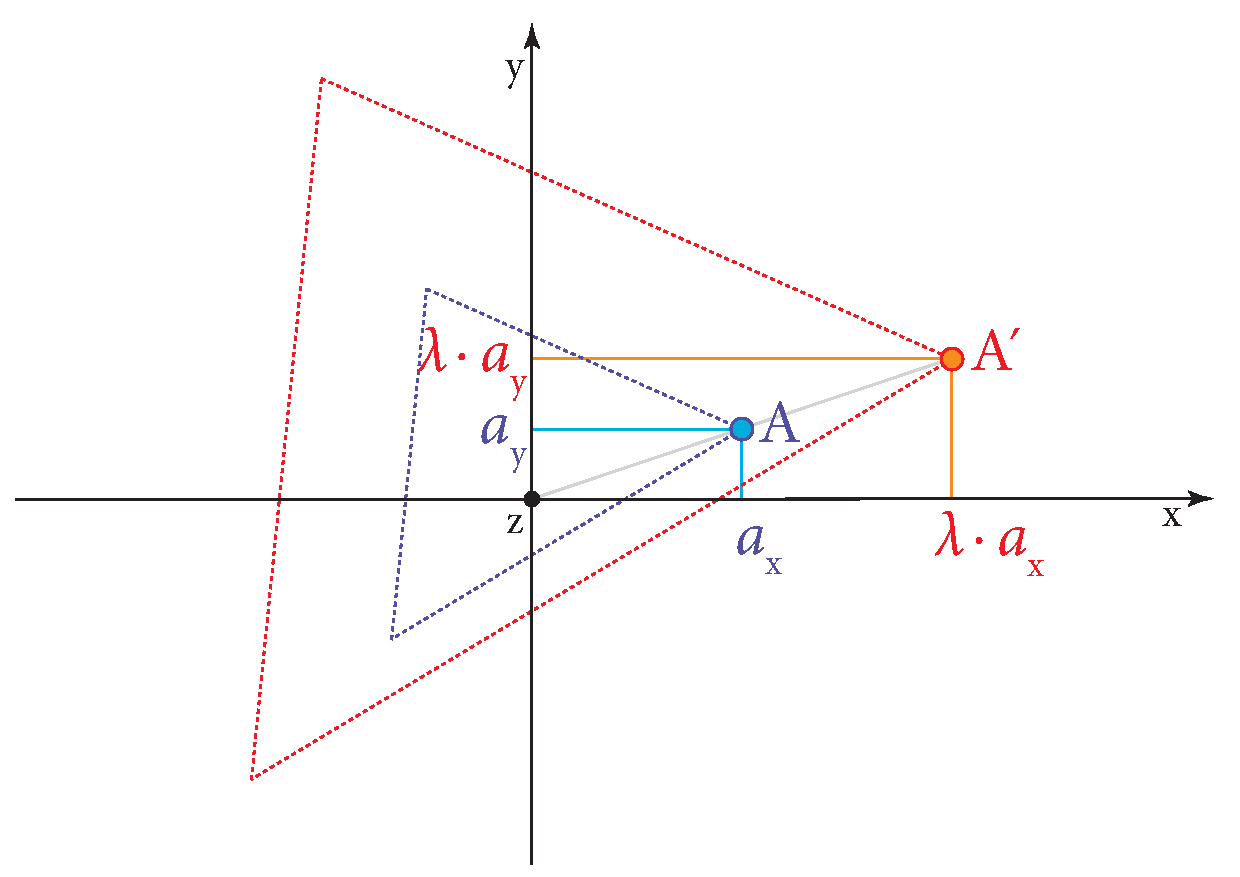
\includegraphics[width=0.49\textwidth]{scaling}
  \vspace{-10pt}
  \caption{Isotrope Skalierung eines Dreiecks um den Faktor $\lambda$.}
\end{wrapfigure}

Die erste und einfachste Transformation, die ich hier vorstellen möchte, ist die Skalierung.

Um ein Objekt zu skalieren, multipliziert man die Koordinaten seiner Eckpunkte jeweils mit einem Skalierungsfaktor $\lambda_i$. Gesucht ist also eine Matrix $S$, für die gilt:
\begin{equation}
 S \cdot
 \begin{pmatrix}
  x \\
  y \\
  z \\
  w
 \end{pmatrix}
 =
 \begin{pmatrix}
  x \cdot \lambda_x \\
  y \cdot \lambda_y \\
  z \cdot \lambda_z \\
  w
 \end{pmatrix}
\end{equation}

Wenn man die Teilgleichung der Multiplikation für eine Koordinate aufstellt (in diesem Fall $x$), erkennt man recht schnell, wie die dazugehörige Zeile der Matrix aussehen muss:
\begin{equation}
\begin{split}
 x \cdot m_{11} + y \cdot m_{12} + z \cdot m_{13} + w \cdot m_{14} = x \cdot \lambda_x \\
 m_{11} = \lambda_x; m_{12} = 0; m_{13} = 0; m_{14} = 0
\end{split}
\end{equation}

Löst man auf die gleiche Weise auch die Teilgleichungen für die anderen Koordinaten, erhält man schließlich folgende Matrix für die \emph{Skalierung um den Koordinatenursprung}:
\begin{equation}
\label{scalingmatrix}
 S{(\lambda_x, \lambda_y, \lambda_z)} =
 \begin{pmatrix}
  \lambda_x & 0 & 0 & 0 \\
  0 & \lambda_y & 0 & 0 \\
  0 & 0 & \lambda_z & 0 \\
  0 & 0 & 0 & 1
 \end{pmatrix}
\end{equation}

Es handelt sich dabei also um eine Diagonalmatrix mit den Skalierungsfaktoren der einzelnen Koordinaten in der Hauptdiagonale (man könnte sie auch als Skalierungsfaktoren der Einheiten der Koordinatenachsen betrachten).

% Quelle: Wikipedia en: Scaling (geometry).
Wenn die Skalierungsfaktoren aller drei Achsen gleich sind, spricht man von einer gleichförmigen oder \emph{isotropen} Skalierung, andernfalls von einer ungleichförmigen oder \emph{antisotropen} Skalierung. Da sich bei einer isotropen Skalierung die Achsen relativ zueinander nicht ändern, sondern auf dreidimensionale Geometrie bezogen nur die Größe des Objektes, wird die isotrope Skalierung zuweilen auch als \emph{Maßstabsänderung} bezeichnet.

Haben alle drei Koeffizienten den Wert $1$, hat die Skalierung keine Auswirkungen -- wie sich leicht überprüfen lässt, ergibt sich aus Gleichung \ref{scalingmatrix} die \emph{Einheitsmatrix}.

Wie man leicht vermuten kann, ist die Skalierung umkehrbar (solange keiner der Faktoren 0 ist). Die inverse Skalierungsmatrix $S^{-1}$ ist dabei die Saklierungsmatrix mit dem Kehrwert der Faktoren:
\begin{equation}
 S^{-1}{(\lambda_x, \lambda_y, \lambda_z)} =
 \begin{pmatrix}
  \frac{1}{\lambda_x} & 0 & 0 & 0 \\
  0 & \frac{1}{\lambda_y} & 0 & 0 \\
  0 & 0 & \frac{1}{\lambda_z} & 0 \\
  0 & 0 & 0 & 1
 \end{pmatrix}
 = S{(\lambda_x^{-1}, \lambda_y^{-1}, \lambda_z^{-1})}
\end{equation}


In manchen Situationen möchte man ein Objekt nicht um den Koordinatenursprung, sondern um einen anderen Punkt im Raum skalieren. In diesem Fall ist die einfachste Lösung, das Objekt zuerst mit einer Translationsmatrix in den Ursprung zu verschieben, die Skalierung durchzuführen und dann das Objekt wieder zurück zu verschieben. Die drei Operationen können in einer Matrix kombiniert werden.

% Matrix 'Skalierung um einen beliebigen Punkt im Raum'?

Sonderfall Spiegelung.

\section{Translation}
\label{translation}

\begin{wrapfigure}{r}{0.5\textwidth}
  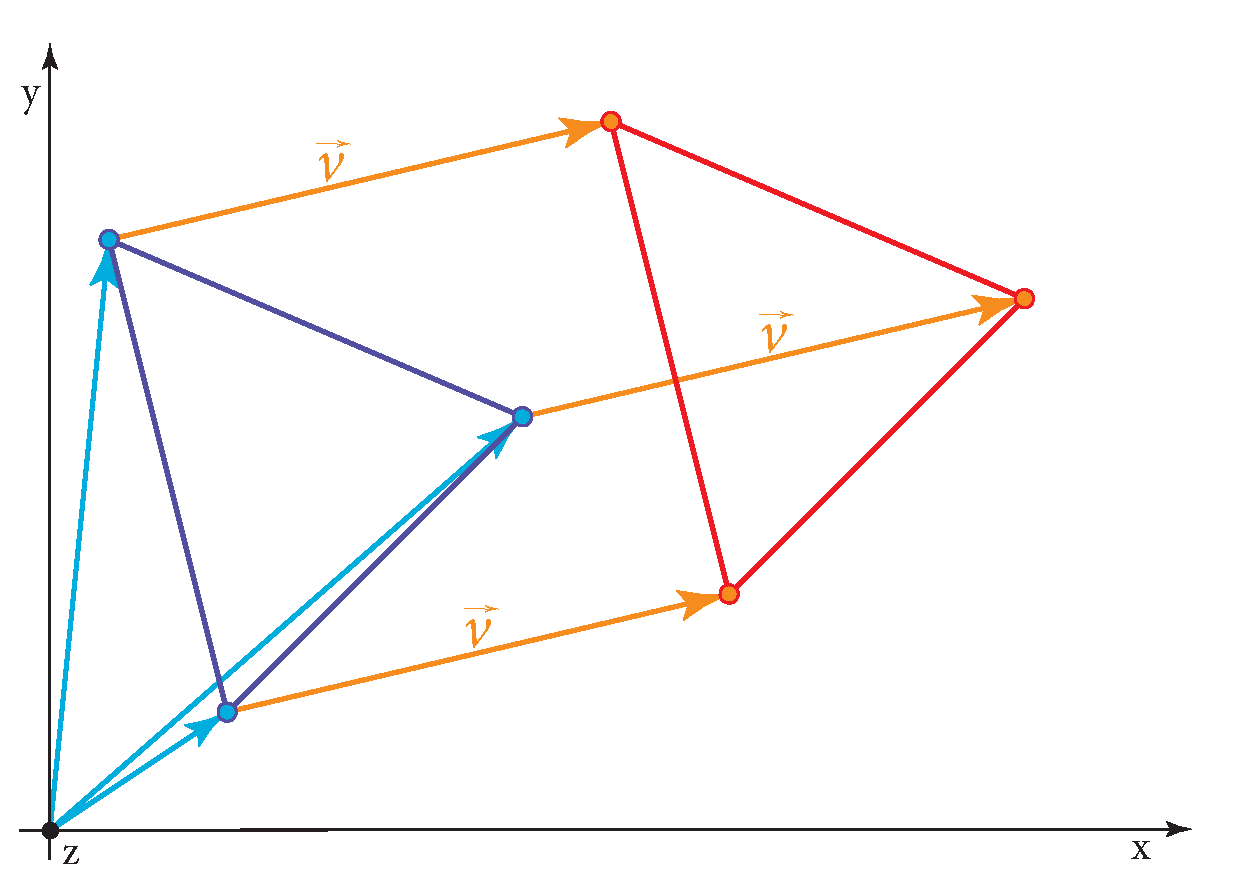
\includegraphics[width=0.49\textwidth]{translation}
  \vspace{-10pt}
  \caption{Translation um $\vec v$.}
\end{wrapfigure}

Die nächste Transformation ist die Translation, also die Verschiebung von Objekten beziehungsweise des Koordinatenursprungs im Raum.

Um alle Eckpunkte eines Objekts um den Vektor $\vec v$ zu verschieben, addiert man die beiden Vektoren einfach nach den Gesetzen der Vektorrechnung komponentenweise. Die gesuchte Translationsmatrix $T$ muss also die folgende Bedingung erfüllen:
\begin{equation}
 T \cdot 
 \begin{pmatrix}
  x \\
  y \\
  z \\
  w
 \end{pmatrix}
 =
 \begin{pmatrix}
  x + v_x \\
  y + v_y \\
  z + v_z \\
  w
 \end{pmatrix}
\end{equation}

Beim Aufstellen der Teilgleichungen (hier exemplarisch für die $y$-Koordinate) wird aber bald ein Problem deutlich:
\begin{equation}
\begin{split}
 x \cdot m_{21} + y \cdot m_{22} + z & \cdot m_{23} + w \cdot m_{24} = y + v_y \\
 m_{21} = 0; m_{23} = & 0; m_{24} = 0 \\
 y \cdot m_{22} & = y + v_y \\
 m_{22} & = \frac{y + v_y}{y} \\
 & = 1 + \frac{v_y}{y}
\end{split}
\end{equation}

Anscheinend gibt es keinen Weg, um die für die Translation nötigen Koeffizienten zu berechnen, ohne die Koordinaten des Vektors zu kennen, der transformiert werden soll. Genau das ist aber Voraussetzung, um die Matrix für mehrere Vektoren verallgemeinern zu können -- die Translation ist offensichtlich keine lineare Transformation!

Der Ausweg aus diesem Dilemma liegt in der Verwendung von homogenen Koordinaten. $w$ hat ja nicht irgendeinen beliebigen Wert, sondern (zumindest vor der Transformation) den Wert 1. Die dementsprechend geänderten Bedingungen für die Translationsmatrix lauten:
\begin{equation}
 T \cdot 
 \begin{pmatrix}
  x \\
  y \\
  z \\
  1
 \end{pmatrix}
 =
 \begin{pmatrix}
  x + v_x \\
  y + v_y \\
  z + v_z \\
  1
 \end{pmatrix}
\end{equation}

Stellt man nun die Teilgleichung für die $y$-Koordinate auf, erhält man:
\begin{equation}
 x \cdot m_{21} + y \cdot m_{22} + z \cdot m_{23} + 1 \cdot m_{24} = y + v_y
\end{equation}

Diese Bedingung ist einfach erfüllt, indem man
\begin{equation}
 m_{21} = 0; m_{22} = 1; m_{23} = 0; m_{24} = v_y
\end{equation}
setzt.

Auf die gleiche Art kann man auch die anderen Teilgleichungen auflösen. Man erhält als Ergebnis die \emph{Translationsmatrix}
\begin{equation}
 T{(\vec v)} =
 \begin{pmatrix}
  1 & 0 & 0 & v_x \\
  0 & 1 & 0 & v_y \\
  0 & 0 & 1 & v_z \\
  0 & 0 & 0 & 1
 \end{pmatrix}.
\end{equation}

So wie die Skalierung ist auch die Translation einfach umkehrbar. Wenn man die inverse Matrix zu der Translationsmatrix $T{(\vec v)}$ berechnet, kommt man dabei auf
\begin{equation}
 T^{-1}{(\vec v)} =
 \begin{pmatrix}
  1 & 0 & 0 & -v_x \\
  0 & 1 & 0 & -v_y \\
  0 & 0 & 1 & -v_z \\
  0 & 0 & 0 & 1
 \end{pmatrix} = T{(-\vec v)},
\end{equation}
also auf die Verschiebung um einen Vektor gleicher Länge in die entgegengesetzte Richtung.

Wie sich leicht zeigen lässt, kann man, um mehrere Translationen nacheinander auf einen Vektor anzuwenden, einfach die einzelnen Verschiebungsvektoren addieren und so eine gemeinsame Matrix erzeugen:
\begin{equation}
 \label{translationaddition}
 T{(\vec a)} \cdot T{(\vec b)} \cdot \vec p = 
 \begin{pmatrix}
  1 & 0 & 0 & a_x + b_x \\
  0 & 1 & 0 & a_y + b_y \\
  0 & 0 & 1 & a_z + b_z \\
  0 & 0 & 0 & 1
 \end{pmatrix} \cdot \vec p = T{(\vec a + \vec b)} \cdot \vec p
\end{equation}

Dieser Zusammenhang mag trivial erscheinen, aber aus Gleichung \ref{translationaddition} ergibt sich noch eine weitere interessante Eigenheit von Translationsmatrizen: Nachdem die Vektoraddition kommutativ ist, mit der man die Translationen zusammenfassen kann, ist auch die \emph{Multiplikation von Translationsmatrizen kommutativ}.

\section{Rotation}
Die Herleitung der dritten und letzten der hier behandelten Transformationen, der Rotation, ist etwas schwieriger als die vorangegangenen. Am einfachsten ist es, sich zunächst auf die Rotation um eine der Koordinatenachsen zu beschränken, im Folgenden wollen wir zunächst die \emph{Rotation um die z-Achse}, also in der \emph{$xy$-Ebene} betrachten.

\subsection{Rotation um die Koordinatenachsen}

\begin{wrapfigure}{r}{0.5\textwidth}
  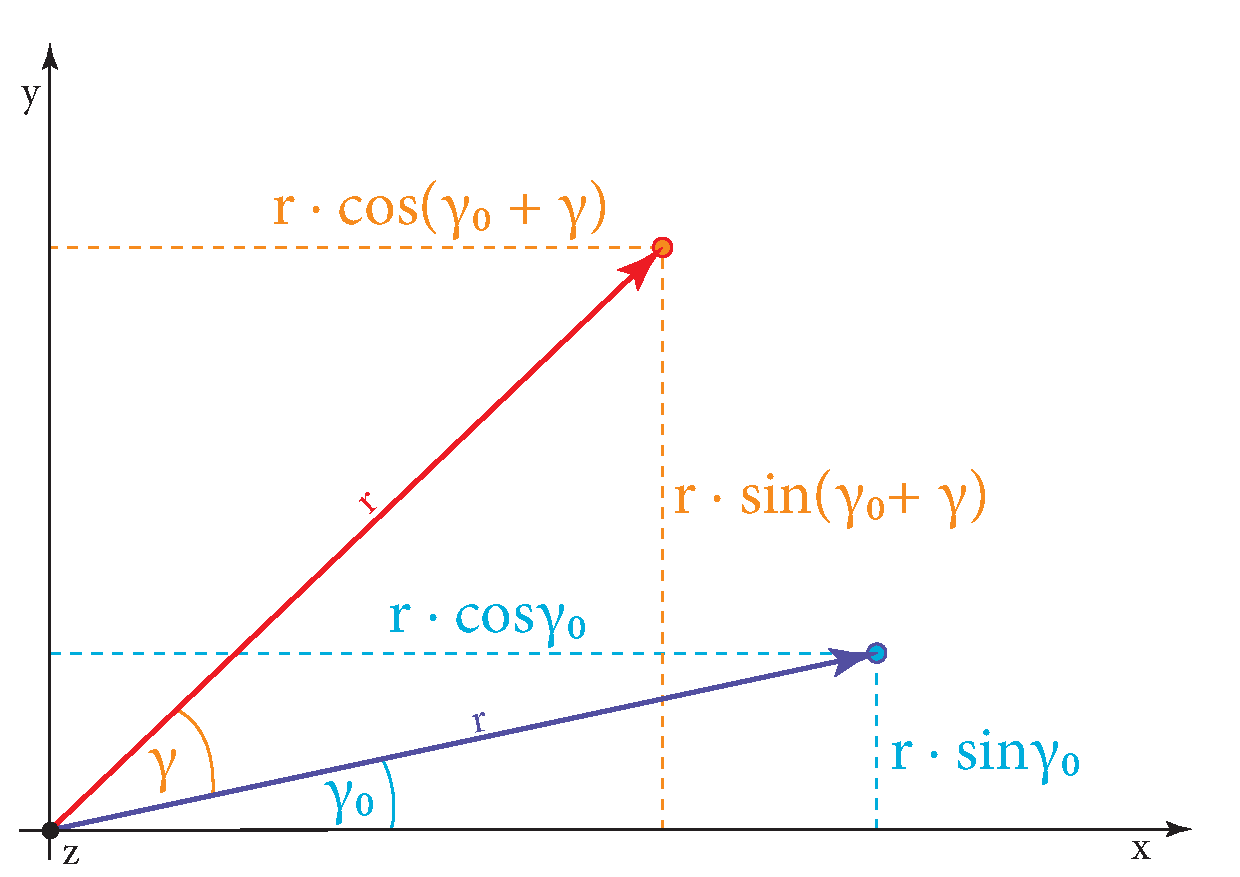
\includegraphics[width=0.49\textwidth]{rotation}
  \vspace{-10pt}
  \caption{Rotation um die $z$-Achse.}
  \label{zrotation}
\end{wrapfigure}

Abbildung \ref{zrotation} zeigt einen Vektor $\vec p = \begin{pmatrix} x & y & z \end{pmatrix}^T$. Nach der Rotation um den Winkel $\gamma$ um die $z$-Achse ergibt sich der Vektor $\vec{p'} = \begin{pmatrix} x' & y' & z' \end{pmatrix}^T$.

Da die Rotation in der $xy$-Ebene stattfindet, ändert sich die $z$-Koordinate des Vektors nicht. Es gilt also
\begin{equation}
 z' = z.
\end{equation}

Für die $x$- und $y$-Koordinaten kann man über die Definition von Sinus und Cosinus ebenfalls direkt aus der Skizze die folgenden Zusammenhänge ableiten:
\begin{align}
  x &= r \cdot \cos{\gamma_0}            &   y &= r \cdot \sin{\gamma_0} \label{rot1} \\
 x' &= r \cdot \cos{(\gamma_0 + \gamma)} &  y' &= r \cdot \sin{(\gamma_0 + \gamma)} \label{rot2}
\end{align}

Unter Zuhilfenahme der trigonometrischen Additionstheoreme erhält man für $x'$ und $y'$ aus \ref{rot2} nach Ausmultiplizieren:
\begin{align}
 \label{rot3}
 x' &= r \cdot \cos \gamma_0 \cos \gamma - r \cdot \sin \gamma_0 \sin \gamma &  y' &= r \cdot \cos \gamma_0 \cos \gamma + r \cdot \sin \gamma_0 \sin \gamma
\end{align}

Die Gleichungen \ref{rot1} ergeben umgeformt:
\begin{align}
 \label{rot4}
 \cos \gamma_0 &= \frac{x}{r} & \sin \gamma_0 &= \frac{y}{r}
\end{align}

Setzt man \ref{rot4} in \ref{rot3} ein, ergibt sich schließlich:
\begin{align}
 x' &= x \cdot \cos \gamma - y \sin \gamma &  y' &= y \cos \gamma + x \sin \gamma
\end{align}

Die gesuchte Rotationsmatrix $R_{z}$ muss also die folgende Bedingung erfüllen:
\begin{equation}
 R_{z} \cdot
 \begin{pmatrix}
  x \\
  y \\
  z \\
  w
 \end{pmatrix}
 = 
 \begin{pmatrix}
  x \cdot \cos \gamma - y \sin \gamma \\
  x \sin \gamma + y \cos \gamma \\
  z \\
  w
 \end{pmatrix}
\end{equation}

Nun ist es ein leichtes, wie für die anderen Transformationen auch die passende Rotationsmatrix für die \emph{Rotation um die $z$-Achse} herzuleiten:
\begin{equation}
 R_z{(\gamma)}
 = 
 \begin{pmatrix}
  \cos \gamma & -\sin \gamma & 0 & 0 \\
  \sin \gamma &  \cos \gamma & 0 & 0 \\
  0 & 0 & 1 & 0 \\
  0 & 0 & 0 & 1 \\
 \end{pmatrix}
\end{equation}

Analog lassen sich auch die Matrizen für die Rotation um die anderen beiden Achsen aufstellen. Man erhält als Ergebnis für die \emph{Rotation um die $x$-Achse}
\begin{equation}
 R_x{(\alpha)}
 = 
 \begin{pmatrix}
  1 & 0 & 0 & 0 \\
  0 & \cos \alpha & -\sin \alpha & 0 \\
  0 & \sin \alpha &  \cos \alpha & 0 \\
  0 & 0 & 0 & 1 \\
 \end{pmatrix}
\end{equation}

und für die \emph{Rotation um die $y$-Achse}
\begin{equation}
 R_y{(\beta)}
 = 
 \begin{pmatrix}
  \cos \beta & 0 & \sin \beta & 0 \\
  0 & 1 & 0 & 0 \\
  -\sin \beta & 0 & \cos \beta & 0 \\
  0 & 0 & 0 & 1 \\
 \end{pmatrix}.
\end{equation}

Jede Rotation lässt sich selbstverständlich durch nochmalige Rotation um den gleichen Betrag in die andere Richtung umkehren. Beim Aufstellen der inversen Matrix
\begin{equation}
 R_z^{-1}{(\gamma)}
 = 
 \begin{pmatrix}
  \cos \gamma & -\sin \gamma & 0 & 0 \\
  \sin \gamma &  \cos \gamma & 0 & 0 \\
  0 & 0 & 1 & 0 \\
  0 & 0 & 0 & 1 \\
 \end{pmatrix}^{-1}
 = 
 \begin{pmatrix}
   \cos \gamma & \sin \gamma & 0 & 0 \\
  -\sin \gamma & \cos \gamma & 0 & 0 \\
  0 & 0 & 1 & 0 \\
  0 & 0 & 0 & 1 \\
 \end{pmatrix}
 = R_z{(-\gamma)}
\end{equation}
fällt einem auf, dass die Inverse der Rotationsmatrix gleich ihrer Transponierten ist. Dies ist auch tatsächlich eine Eigenheit aller Rotationsmatrizen, beziehungsweise aller Transformationen, bei denen eine beliebige Länge erhalten bleibt.
%Beweis von http://mathworld.wolfram.com/RotationMatrix.html

\subsection{Eulersche Winkel}
Die gerade behandelten Rotationsmatrizen sind auf Drehungen um die Koordinatenachsen beschränkt, aber natürlich lassen sich mehrere der Matrizen kombinieren, um jede beliebige Rotation ausdrücken zu können.

Ein beliebtes Verfahren, um Ausrichtungen im Raum anzugeben, sind die sogenannten Eulerschen Winkel. Dabei handelt es sich um drei Rotationswinkel um jeweils eine Achse, durch die jede beliebige Rotation ausgedrückt werden kann. Es gibt mehrere Konventionen, in welcher Reihenfolge die Rotationen auf welche Achsen angewendet werden. Eine der am häufigsten benutzten sind die aus der Luftfahrt bekannten \emph{Roll-Nick-Gier-Winkel}, auch als \emph{Tait–Bryan-Rotation} bezeichnet (engl. \emph{yaw, pitch, roll}). Sie geben die Rotation als Kombination einer Rotation um die $z$-Achse ($\gamma$), gefolgt von einer Rotation um die $y$-Achse ($\beta$) und schließlich einer Rotation um die $x$-Achse ($\alpha$) an.

Mit einem Wertebereich von $-\pi$ bis $\pi$ für $\alpha$ und $\gamma$ und von $-\frac{\pi}{2}$ bis $\frac{\pi}{2}$ für $\beta$ lassen sich alle Ausrichtungen im Raum angeben. Bis auf zwei Ausnahmen (dazu gleich mehr) ist auch jedem Rotationszustand genau ein Satz an Winkeln zugeordnet, die Abbildung ist also bis auf ebendiese Ausnahmen bijektiv.

Um eine Rotationsdarstellung in Eulerschen Winkeln in Matrixform zu überführen, muss man einfach die Rotationsmatrizen für die einzelnen Achsen miteinander multiplizieren:

\begin{equation}
\begin{split}
 &R_{zyx}( \gamma, \beta, \alpha ) = R_x( \alpha ) \cdot R_y( \beta ) \cdot R_z( \gamma ) \\
 &=
 \begin{pmatrix}
  1 & 0 & 0 & 0 \\
  0 & \cos \alpha & -\sin \alpha & 0 \\
  0 & \sin \alpha &  \cos \alpha & 0 \\
  0 & 0 & 0 & 1 \\
 \end{pmatrix} \cdot
 \begin{pmatrix}
  \cos \beta & 0 & \sin \beta & 0 \\
  0 & 1 & 0 & 0 \\
  -\sin \beta & 0 & \cos \beta & 0 \\
  0 & 0 & 0 & 1 \\
 \end{pmatrix} \cdot
 \begin{pmatrix}
  \cos \gamma & -\sin \gamma & 0 & 0 \\
  \sin \gamma &  \cos \gamma & 0 & 0 \\
  0 & 0 & 1 & 0 \\
  0 & 0 & 0 & 1 \\
 \end{pmatrix} \\
 &=
 \begin{pmatrix}
  \cos \beta \cos \gamma & \cos \beta \sin \gamma & - \sin \beta & 0 \\
  \sin \alpha \sin \beta \cos \gamma - \cos \alpha \sin \gamma & \sin \alpha \sin \beta \sin \gamma + \cos \alpha \cos \gamma & \sin \alpha \cos \beta & 0\\
  \cos \alpha \sin \beta \cos \gamma + \sin \alpha \sin \gamma & \cos \alpha \sin \beta \sin \gamma - \sin \alpha \cos \gamma & \cos \alpha \cos \beta & 0\\
  0 & 0 & 0 & 1
 \end{pmatrix}
\end{split}
\end{equation}

Eulersche Winkel sind ein vergleichbar einfaches und intuitives Mittel, um beliebige Rotationen anzugeben, und werden in der 3D-Grafik gerne für statische Angaben von Rotationen verwendet. Im Bezug auf Animationen haben sie jedoch einige Nachteile:

Zum einen ist es schwer, zwischen zwei in Eulerschen Winkeln gegebenen Rotationszuständen so zu interpolieren, dass die Winkelgeschwindigkeit der resultierenden Rotationsbewegung konstant bleibt. Dies ist für manche Anwendungen wünschenswert, etwa Kamerafahrten, damit die Animation flüssig erscheint.

Zum anderen gibt es wie schon erwähnt für die Zuordnung von Eulerschen Winkeln zu Rotationen zwei kritische Punkte, im Falle der $zyx$-Konvention bei $\beta = \pm \frac{\pi}{2}$, also bei einer Rotation von $90^\circ$ um die $y$-Achse. Setzt man $\frac{\pi}{2}$ in die Matrix ein, erhält man
\begin{equation}
\begin{split}
 R_{zyx}{\left(\alpha, \frac{\pi}{2}, \gamma \right)}
 & = 
 \begin{pmatrix}
  0 & 0 & -1 & 0 \\
  \sin \alpha \cos \gamma - \cos \alpha \sin \gamma & \sin \alpha \sin \gamma + \cos \alpha \cos \gamma & 0 & 0 \\
  \cos \alpha \cos \gamma + \sin \alpha \sin \gamma & \cos \alpha \sin \gamma - \sin \alpha \cos \gamma & 0 & 0 \\
  0 & 0 & 0 & 1
 \end{pmatrix} \\
 & = 
 \begin{pmatrix}
  0 & 0 & -1 & 0 \\
  \sin ( \alpha - \gamma ) &  \cos ( \alpha - \gamma ) & 0 & 0 \\
  \cos ( \alpha - \gamma ) & -\sin ( \alpha - \gamma ) & 0 & 0 \\
  0 & 0 & 0 & 1
 \end{pmatrix}
\end{split}
\end{equation}

Die Rotation hängt nun ausschließlich von der Differenz $\alpha - \gamma$ ab -- das System hat einen Freiheitsgrad eingebüßt! Es gibt jetzt unendlich viele Kombinationen von $\alpha$ und $\gamma$, die zu der gleichen Ausrichtung im Raum führen; die Abbildung der Eulerschen Winkel auf die Rotationsmatrizen ist also nicht injektiv.

Dieses Problem tritt auch bei kardanischen Aufhängungen in der Mechanik auf, beispielsweise bei Trägheitsnavigationssystemen\footnote{Ein echtes Problem ist der Gimbal Lock in der Raumfahrt, wo die kardanische Aufhängung tatsächlich Drehungen um alle drei Freiheitsgrade kompensieren muss. (\vgl irgendein NASA-Dokument)}. Es wird daher als \emph{Gimbal Lock} bezeichnet (engl. \emph{gimbal} bezeichnet einen Kardanring, zu Deutsch also etwa Kardanring-Blockade). In der Mechanik hat man oft die Möglichkeit, Situationen, die zu einem Gimbal Lock führen können, rechtzeitig zu erkennen und den Gimbal Lock zu vermeiden, etwa durch Änderung des Flugmanövers. Bei vom Benutzer ausgelösten oder gesteuerten Rotationen in Computerprogrammen ist dies aber kaum möglich, dewegen greift man normalerweise auf andere Verfahren zurück zurück, um Rotationen zu speichern und zu verarbeiten.
% Picture 'Gimbal lock in mechanics'?

\subsection{Herleitung über transformierte Basisvektoren}
\label{rotationbasevectors}
In den vorigen beiden Abschnitten haben wir die Konstruktion einer Rotationsmatrix ausgehend von einem oder mehreren Rotationswinkeln besprochen. In manchen Fällen kennt man aber bereits die \emph{Basisvektoren} des neuen Koordinatensystems (in den Koordinaten des alten Systems) und will eine Matrix aufstellen, um alle anderen Vektoren zu transformieren.

Hat man drei linear unabhängige Vektoren im alten und im neuen (dreidimensionalen) Koordinatensystem gegeben, lässt sich die Transformationsmatrix $T$ für jede lineare Transformation bestimmen, indem man die Vektoren in die Gleichung $\vec{v'} = T \cdot \vec v$ einsetzt und das Gleichungssystem löst. Daraus ergeben sich allerdings neun Gleichungen in neun Variablen -- händisch eine nervige und für den Computer eine relativ rechenaufwändige Angelegenheit. Kennt man aber die transformierten \emph{kanonischen Basisvektoren}, $\begin{pmatrix} 1 & 0 & 0 \end{pmatrix}^T$, $\begin{pmatrix} 0 & 1 & 0 \end{pmatrix}^T$ und $\begin{pmatrix} 0 & 0 & 1 \end{pmatrix}^T$, vereinfachen sich die Gleichungen wesentlich:

\begin{equation}
 T \cdot \begin{pmatrix} 1 \\ 0 \\ 0 \end{pmatrix} = \begin{pmatrix} x_x \\ x_y \\ x_z \end{pmatrix} \qquad 
\begin{aligned}
 1 \cdot t_{11} + 0 \cdot t_{12} + 0 \cdot t_{13} = t_{11} &= x_x \\
 1 \cdot t_{21} + 0 \cdot t_{22} + 0 \cdot t_{23} = t_{21} &= x_y \\
 1 \cdot t_{31} + 0 \cdot t_{32} + 0 \cdot t_{33} = t_{31} &= x_z
\end{aligned}
\end{equation}

\begin{equation}
 T \cdot \begin{pmatrix} 0 \\ 1 \\ 0 \end{pmatrix} = \begin{pmatrix} y_x \\ y_y \\ y_z \end{pmatrix} \qquad
\begin{aligned}
 0 \cdot t_{11} + 1 \cdot t_{12} + 0 \cdot t_{13} = t_{12} &= y_x \\
 0 \cdot t_{21} + 1 \cdot t_{22} + 0 \cdot t_{23} = t_{22} &= y_y \\
 0 \cdot t_{31} + 1 \cdot t_{32} + 0 \cdot t_{33} = t_{32} &= y_z
\end{aligned}
\end{equation}

\begin{equation}
 T \cdot \begin{pmatrix} 0 \\ 0 \\ 1 \end{pmatrix} = \begin{pmatrix} z_x \\ z_y \\ z_z \end{pmatrix} \qquad
\begin{aligned}
 0 \cdot t_{11} + 0 \cdot t_{12} + 1 \cdot t_{13} = t_{13} &= z_x \\
 0 \cdot t_{21} + 0 \cdot t_{22} + 1 \cdot t_{23} = t_{23} &= z_y \\
 0 \cdot t_{31} + 0 \cdot t_{32} + 1 \cdot t_{33} = t_{33} &= z_z
\end{aligned}
\end{equation}

Für die drei neuen Basisvektoren $\vec x$, $\vec y$ und $\vec z$ entsteht also die Matrix
\begin{equation}
 T(\vec x, \vec y, \vec z) =
 \begin{pmatrix}
  x_x & y_x & z_x \\
  x_y & y_y & z_y \\
  x_z & y_z & z_z \\
 \end{pmatrix},
\end{equation}
beziehungsweise für die Verwendung mit homogenen Koordinaten
\begin{equation}
 T(\vec x, \vec y, \vec z) =
 \begin{pmatrix}
  x_x & y_x & z_x & 0 \\
  x_y & y_y & z_y & 0 \\
  x_z & y_z & z_z & 0 \\
  0 & 0 & 0 & 1
 \end{pmatrix}.
\end{equation}

In Worten ausgedrückt, enthält eine Transformationsmatrix also in ihren Spalten die \emph{Bilder der kanonischen Basisvektoren}.

\subsection{Darstellung als Quaternion}
Wie schon bei der Einführung der Quaternionen in Kapitel \ref{quaternionmath} erwähnt, können Quaternionen als Verbindung eines Skalars und eines dreidimensionalen Vektors aufgefasst werden, wobei der Realteil $w$ den Skalar und der Imaginärteil $xi + yj + zk$ den Vektor $\begin{pmatrix}x & y & z\end{pmatrix}^T$ darstellt. Sie eigenen sich deshalb gut für die Darstellung einer Rotation um einen bestimmten Winkel um eine beliebige Achse -- der Rotationswinkel entspricht dem Realteil, die Rotationsachse dem Imaginärteil.

Um mit der Hilfe von Quaternionen die Rotation eines Vektors $\vec x$ um den Winkel $2 \phi$ mit der Achse $\vec n$ durchzuführen, bildet man zunächst die Quaternion $q = \left[ \cos \phi; \vec n \cdot \sin \phi \right]$. Das Ergebnis der Rotation lautet dann $q \cdot \hat{x} \cdot \overline{q}$. Der Vektor $\vec x$ wird hier, wie in Kapitel \ref{quaternionmath} besprochen, als reine Quaternion behandelt. Das Ergebnis der Berechnung ist ebenfalls wieder eine reine Quaternion, kann also wieder als dreidimensionaler Vektor aufgefasst werden. So lautet die Rotationsformel (mit $\left| n \right| = 1$) schließlich:
\begin{equation}
 \hat{x}' = \left[ \cos \phi; \vec n \cdot \sin \phi \right] \cdot \hat{x} \cdot \left[ \cos \phi; -\vec n \cdot \sin \phi \right]
\end{equation}

\begin{wrapfigure}{r}{0.5\textwidth}
  \vspace{-10pt}
  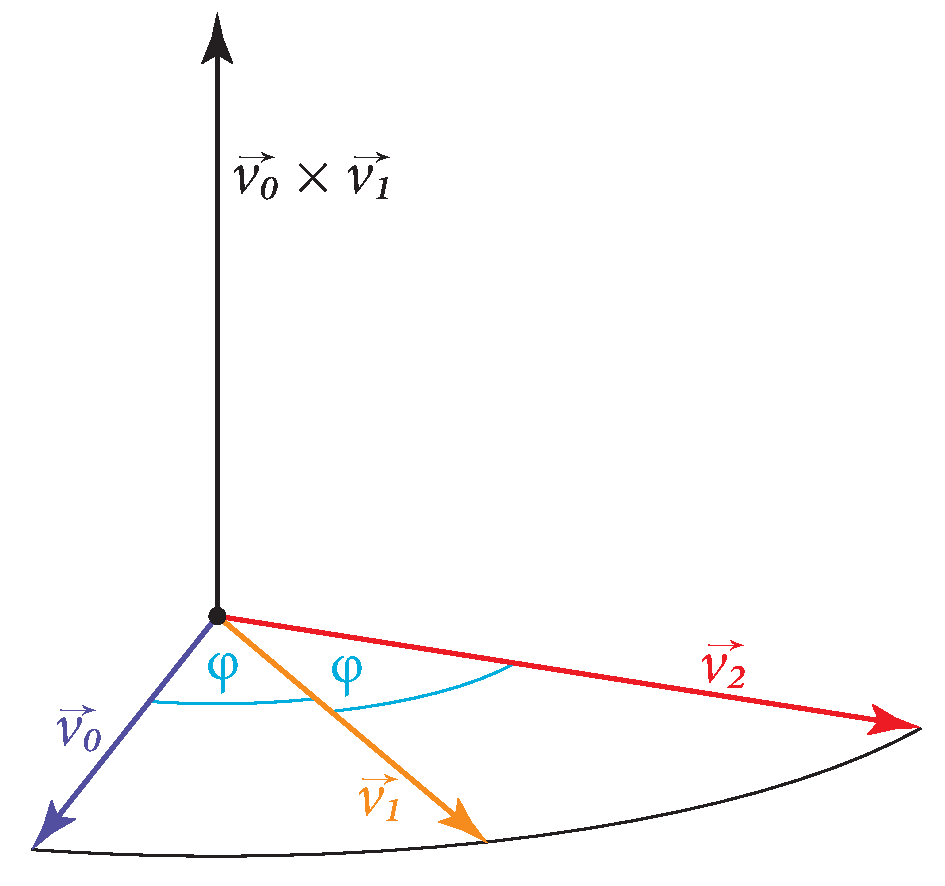
\includegraphics[width=0.49\textwidth]{quatrotation}
  \vspace{-10pt}
  \caption{Rotation um die Achse $\vec{v_0} \times \vec{v_1}$.}
\end{wrapfigure}

Um zu beweisen, dass die oben abgebildete Formel wirklich eine Rotation des Vektors darstellt, betrachten wir zunächst einmal drei Einheitsvektoren $\vec{v_0}$, $\vec{v_1}$ und $\vec{v_2}$ aus dem $\mathbb R^3$ (\vgl \citep{quaternionproof}). Sie sind koplanar und bilden jeweils den Winkel $\phi$. Es gilt daher:
\begin{align}
 \vec{v_0} \cdot \vec{v_1} = \vec{v_1} \cdot \vec{v_2} = \cos \phi \label{dotsame} \\
 \vec{v_0} \times\vec{v_1} = \vec{v_1} \times \vec{v_2} \label{crosssame}
\end{align}
$\vec{v_2}$ ensteht also durch eine Rotation von $\vec{v_0}$ um den Winkel $2 \phi$ mit der Achse $\vec{v_0} \times \vec{v_1}$.

Wir definieren nun die Quaternion $q$ über $\vec{v_0}$ und $\vec{v_1}$:
\begin{equation}
 q = \left[ \left( \vec{v_0} \cdot \vec{v_1} \right); \vec{v_0} \times \vec{v_1} \right]
\end{equation} 

Wir wollen zunächst beweisen:
\begin{equation}
 \label{quaternionclaim}
 q \cdot \hat{v_0} \cdot \overline{q} = p_2
\end{equation} 

Für $q$ gilt
\begin{equation}
 \label{equality1}
 q = \hat{v_1} \cdot \overline{\hat{v_0}},
\end{equation}
weil nach der Multiplikationsvorschrift für Quaternionen (siehe Gleichung \ref{quaternionmultiplicationvector}) gilt:
\begin{equation}
\begin{split}
 \hat{v_1} \cdot \overline{\hat{v_0}} &= \left[ \left( 0 - \vec{v_1} \cdot (-\vec{v_0}) \right); \vec{v_1} \times (-\vec{v_0}) + 0 \cdot (-\vec{v_0}) + 0 \cdot \vec{v_1} \right] \\
 &= \left[ \vec{v_1} \cdot \vec{v_0}; -( \vec{v_1} \times \vec{v_0}) \right] \\
 &= \left[ \vec{v_0} \cdot \vec{v_1}; \vec{v_0} \times \vec{v_1} \right]
\end{split}
\end{equation} 

Dann gilt natürlich auch
\begin{equation}
 \label{equality2}
 q = \hat{v_2} \cdot \overline{\hat{v_1}},
\end{equation} 
weil ja nach Gleichung \ref{dotsame} und \ref{crosssame} die Skalar- und Kreuzprodukte der beiden Vektorenpaare identisch sind.

Wir setzen nun den Zusammenhang aus \ref{equality1} in Gleichung \ref{quaternionclaim} ein und erhalten:
\begin{equation}
\begin{split}
 \label{step1}
 \hat{v_1} \cdot \overline{\hat{v_0}} \cdot \hat{v_0} \cdot \overline{q} &= \hat{v_2} \\
 \hat{v_1} \cdot \left| \hat{v_0} \right| \cdot \overline{q} &= \hat{v_2}
\end{split}
\end{equation}

Nachdem $v_0$ ein Einheitsvektor ist, hat auch $\hat{v_0}$ den Betrag 1, der Ausdruck vereinfacht sich also zu:
\begin{equation}
 \hat{v_1} \cdot \overline{q} = \hat{v_2}
\end{equation}

Nun setzen wir den Zusammenhang aus \ref{equality2} für $\overline{q}$ ein und vereinfachen nach Gleichung \ref{quaternionconjugationmultiplication}:
\begin{equation}
\begin{split}
 \label{step2}
 \hat{v_1} \cdot \overline{\left( \hat{v_2} \cdot \overline{\hat{v_1}} \right)} &= \hat{v_2} \\
 \hat{v_1} \cdot \hat{v_1} \cdot \overline{\hat{v_2}} &= \hat{v_2}
\end{split}
\end{equation}

Nachdem $\hat{v_1}$ eine reine Quaternion und $v_1$ ein Einheitsvektor ist, vereinfacht sich der Ausdruck $\hat{v_1} \cdot \hat{v_1}$:
\begin{equation}
\begin{split}
 \hat{v_1} \cdot \hat{v_1} &= \left[ \left( 0 - \vec{v_1} \cdot \vec{v_1} \right); \vec{v_1} \times \vec{v_1} + 0 \cdot \vec{v_1} + 0 \cdot \vec{v_1} \right] \\
 &= \left[ -\left| \vec{v_1} \right|; \vec 0 \right] \\
 &= -1
\end{split}
\end{equation}

Wir setzen in \ref{step2} ein und erhalten:
\begin{equation}
\begin{split}
 -\overline{\hat{v_2}} &= \hat{v_2} \\
 -\left[ 0; -\vec{v_2} \right] &= \left[ 0; \vec{v_2} \right] \\
 \vec{v_2} &= \vec{v_2}
\end{split}
\end{equation}

Damit wäre der Zusammenhang aus Gleichung \ref{quaternionclaim} bewiesen:
\begin{equation*}
 q \cdot \hat{v_0} \cdot \overline{q} = \hat{v_2}
\end{equation*}

Für $q$ eingesetzt:
\begin{equation*}
 \left[ ( \vec{v_0} \cdot \vec{v_1} ); \vec{v_0} \times \vec{v_1} \right] \cdot \hat{v_0} \cdot \left[ ( \vec{v_0} \cdot \vec{v_1} ); -(\vec{v_0} \times \vec{v_1} ) \right] = \hat{v_2}
\end{equation*} 

Unter Beachtung der Zusammenhänge $\vec a \cdot \vec b = \left| a \right| \cdot \left| b \right| \cdot \cos \phi$ und $\left| \vec a \times \vec b \right| = \left| a \right| \cdot \left| b \right| \cdot \sin \phi$ und der Tatsache, dass $\vec{v_0}$ und $\vec{v_1}$ Einheitsvektoren sind, können wir nun einsetzen:
\begin{equation}
 \left[ \cos \phi; \vec n \cdot \sin \phi \right] \cdot \hat{v_0} \cdot \left[ \cos \phi; -\vec n \cdot \sin \phi \right] = \hat{v_2}
\end{equation}

Nun brauchen wir nur noch beide Seiten mit einem beliebigen Skalar $a$ zu multiplizieren ($\hat{v_0}$ und $\hat{v_2}$ sind ja auf Einheitsquaternionen beschränkt), und es ergibt sich:
\begin{equation}
\begin{split}
 \left[ \cos \phi; \vec n \cdot \sin \phi \right] \cdot a \cdot \hat{v_0} \cdot \left[ \cos \phi; -\vec n \cdot \sin \phi \right] &= a \cdot \hat{v_2} \\
 \left[ \cos \phi; \vec n \cdot \sin \phi \right] \cdot \hat{x} \cdot \left[ \cos \phi; -\vec n \cdot \sin \phi \right] &= \hat{x}'
\end{split}
\end{equation}

Wenn die Quaternionen $q_1, q_2, \ldots, q_n$ eine Rotation darstelen, dann lassen sich die Rotationen in eine Quaternion $q$ kombiniern, indem man die Quaterionen -- ähnlich wie bei Transformationsmatrizen -- einfach miteinander multipliziert: $q = q_n \cdot q_{n-2} \cdot \ldots \cdot q_1$. Der zugehörige Beweis ist nahezu trivial: Rotationen zu verketten heißt ja, das Ergebnis der einen Rotation als Ausgangswert für die nächste Transformation zu verwenden. Im Falle von drei Rotationen lautet die Formel also
\begin{equation}
 \hat{x}' = q_3 \cdot ( q_2 \cdot ( q_3 \cdot \hat{x} \cdot \overline{q_1} ) \cdot \overline{q_2} ) \cdot \overline{q_3},
\end{equation}
was wir wegen der Assoziativität der Quaternionenmultiplikation als 
\begin{equation}
 \hat{x}' = ( q_3 \cdot q_2 \cdot q_1 ) \cdot \hat{x} \cdot ( \overline{q_1} \cdot \overline{q_2} \cdot \overline{q_3} )
\end{equation}
schreiben können, was wir gleich zu
\begin{equation}
\begin{split}
 \hat{x}' &= ( q_3 \cdot q_2 \cdot q_1 ) \cdot \hat{x} \cdot \overline{( q_3 \cdot q_2 \cdot q_1 )} \\
 &= q \cdot \hat{x} \cdot \overline{q}
\end{split}
\end{equation} 
vereinfachen können, da sich die Quaternionenmultiplikation ja bezüglich der Konjugation distributiv unter Vertauschung der Reihenfolge verhält (siehe Gleichung \ref{quaternionconjugationmultiplication}).

Quaternionen stellen also wegen ihrer Beziehung zu Rotationswinkel und -achse ein praktisches Mittel dar, um Rotationen anzugeben und mehrere Rotationen können einfach miteinander kombiniert werden (auch im Bezug auf die benötigten Rechenoperationen am Computer). Zusätzlich kann es für manche Computeranwendungen nützlich sein, dass nur vier Werte gespeichert werden müssen, um jede beliebige Rotation darzustellen. Die Repräsentation als Quaternion hat aber auch Nachteile. Zum einen ist die direkte Transformation von Vektoren durch Quaternionen eine relativ rechenaufwändige Angelegenheit, was für den Einsatz in der 3D-Grafik nicht gerade optimal ist. Zum anderen unterstützt die derzeitige Grafikhardware wie in Kapitel \ref{coordinatesystems} beschrieben lediglich Matrizen, um die Vertices zu transformieren. Daher liegt es nahe, einen Weg zu suchen, eine Rotationsquaternion in eine Rotationsmatrix zu konvertieren. (\vgl \citep{rotationissues}, 8-9)

Nachdem ja $\hat{x}'= q \cdot \hat{x} \cdot \overline{q}$ gilt, liegt es nahe, dass man auch nach einer Matrix suchen kann, für die $\vec{x}' = M \cdot \vec{x}$ gilt, die also bei entsprechender Interpretation von reinen Quaternionen als Vektoren die Bedingung $q \cdot \hat{x} \cdot \overline{q} = M \cdot \vec{x}$ erfüllt. Es gibt zahlreiche Wege, die Matrix direkt aus diesem Zusammenhang herzuleiten (\vgl \citep{quaternionrotation}, 56-58; \citep{script:spain}, 93-96), ich möchte aber stattdessen eine andere Möglichkeit zur Herleitung anführen, die leichter nachzuvollziehen ist.

Wie in Abschnitt \ref{rotationbasevectors} besprochen, kann man eine Transformationsmatrix als Aneinanderreihung der transformierten kanonischen Basisvektoren aufstellen. Um eine Matrix aus einem Rotationsquaternion zu erzeugen, muss man also nur die drei Basisvektoren direkt transformieren und die Ergebnisse in die Matrix schreiben.

Dafür multiplizieren wir zunächst einmal die Rotationsformel aus und vereinfachen (\vgl \citep{quaternionrotation}, 52):
\begin{equation}
\begin{split}
 q \cdot \hat{x} \cdot \overline{q} &= \left[ w; \vec n \right] \cdot \left[ 0; \vec x \right] \cdot \left[ w; -\vec n \right] \\
 &= \left[ - \vec n \cdot \vec x; \vec n \times \vec x + w \cdot \vec x \right] \cdot \left[ w; -\vec n \right] \\
 &= \begin{split}[ &- w \cdot ( \vec n \cdot \vec x ) + ( \vec n \times \vec x + w \cdot \vec x ) \cdot \vec n; \\
  &- ( \vec n \times \vec x + w \cdot \vec x ) \times \vec n + w \cdot ( \vec n \times \vec x + w \cdot \vec x ) - \vec n \cdot \vec x \cdot ( - \vec n ) ] \end{split} \\
 &= \begin{split}[ &- w \cdot ( \vec n \cdot \vec x ) + ( \vec n \times \vec x ) \cdot \vec n + w \cdot ( \vec n \cdot \vec x ); \\
  &- ( ( \vec n \times \vec x ) \times \vec n ) - w \cdot ( \vec x \times \vec n ) + w \cdot ( \vec n \times \vec x ) + w^2 \cdot \vec x + ( \vec n \cdot \vec x ) \cdot \vec n ] \end{split} \\
 &= \left[ 0; \vec n \times ( \vec n \times \vec x ) + 2 \cdot w \cdot ( \vec n \times \vec x ) + w^2 \cdot \vec x + ( \vec n \cdot \vec x ) \cdot \vec n \right] \\
 &= \left[ 0; 2 \cdot ( \vec n \cdot \vec x ) \cdot \vec n + 2 \cdot w \cdot ( \vec n \times \vec x ) + ( w^2 - \vec n \cdot \vec n ) \cdot \vec x \right]
\end{split}
\end{equation}

Mithilfe dieser Formel transformieren wir nun die drei Basisvektoren $\vec x$, $\vec y$ und $\vec z$. Für die Komponenten von $\vec x$ erhalten wir:
\begin{equation}
\begin{split}
 x_x' &= 2 \cdot ( x + 0 + 0 ) \cdot x + 2 \cdot w \cdot ( y \cdot 0 - z \cdot 0 ) + ( w^2 - x^2 - y^2 - z^2 ) \cdot 1 \\
      &= x^2 + w^2 - y^2 - z^2 \\
      &= ( 1 - y^2 - z^2 - w^2 ) + w^2 - y^2 - z^2 \\
      &= 1 - 2 \cdot ( y^2 + z^2 )
\end{split}
\end{equation}
\begin{equation}
\begin{split}
 x_y' &= 2 \cdot ( x + 0 + 0 ) \cdot y + 2 \cdot w \cdot ( 1 \cdot z - 0 \cdot x ) + ( w^2 - x^2 - y^2 - z^2 ) \cdot 0 \\
      &= 2xy + 2wz \\
      &= 2 \cdot ( xy + wz )
\end{split}
\end{equation}
\begin{equation}
\begin{split}
 x_z' &= 2 \cdot ( x + 0 + 0 ) \cdot z + 2 \cdot w \cdot ( x \cdot 0 - y \cdot 1 ) + ( w^2 - x^2 - y^2 - z^2 ) \cdot 0 \\
      &= 2xz - 2wy \\
      &= 2 \cdot ( xz + wy )
\end{split}
\end{equation}

Analog werden auch die anderen beiden Vektoren transformiert:
\begin{align}
 \vec{y'} =
 \begin{pmatrix}
  2 \cdot ( xy - wz ) \\
  1 - 2 \cdot ( x^2 + z^2 ) \\
  2 \cdot ( yz + wx )
 \end{pmatrix} \\
 \vec{z'} = 
 \begin{pmatrix}
  2 \cdot ( xz + wy ) \\
  2 \cdot ( yz - wx ) \\
  1 - 2 \cdot ( x^2 + y^2 )
 \end{pmatrix}
\end{align}

Durch Nebeneineinanderstellen von $\vec{x'}$, $\vec{y'}$ und $\vec{z'}$ ergibt sich schließlich \emph{Rotationsmatrix zu einer Rotationsquaternion $q = w + xi + yj + zk$}
\begin{equation}
 R(q) =
 \begin{pmatrix}
  1 - 2 \cdot ( y^2 + z^2 ) & 2 \cdot ( xy - wz ) & 2 \cdot ( xz + wy ) \\
  2 \cdot ( xy + wz ) & 1 - 2 \cdot ( x^2 + z^2 ) & 2 \cdot ( yz - wx ) \\
  2 \cdot ( xz - wy ) & 2 \cdot ( yz + wx ) & 1 - 2 \cdot ( x^2 + y^2 )
 \end{pmatrix},
\end{equation}
beziehungsweise zur Verwendung mit homogenen Koordinaten
\begin{equation}
 R(q) =
 \begin{pmatrix}
  1 - 2 \cdot ( y^2 + z^2 ) & 2 \cdot ( xy - wz ) & 2 \cdot ( xz + wy ) & 0 \\
  2 \cdot ( xy + wz ) & 1 - 2 \cdot ( x^2 + z^2 ) & 2 \cdot ( yz - wx ) & 0 \\
  2 \cdot ( xz - wy ) & 2 \cdot ( yz + wx ) & 1 - 2 \cdot ( x^2 + y^2 ) & 0 \\
  0 & 0 & 0 & 1
 \end{pmatrix}.
\end{equation}

%\subsection{SLERP und andere Interpolationsverfahren}